\documentclass{article}
%% PACKAGES %%

\usepackage{amsmath, amsfonts, amssymb, amsthm}
\usepackage{braket}
\usepackage{listings}
\usepackage{geometry}
\usepackage{xcolor}
\usepackage{textcomp}
\usepackage{graphicx}
\usepackage{fancyhdr}
\usepackage{sourcecodepro}
\usepackage{multirow}

%%%%%%%%%%%%%%

\graphicspath{{./images}}
\setlength\parindent{0pt}       % globally supress indentation

%% LISTINGS CONFIG %%

\definecolor{purple2}{RGB}{153,0,153} % there's actually no standard purple
\definecolor{green2}{RGB}{0,153,0} % a darker green

\lstset{
  language=MATLAB,                   % the language
  basicstyle=\normalsize\ttfamily,   % size of the fonts for the code
  frame = single,
  % Color settings to match IDLE style
  keywordstyle=\color{orange},       % core keywords
  keywordstyle={[2]\color{purple2}}, % built-ins
  stringstyle=\color{green2},%
  showstringspaces=false,
  commentstyle=\color{red},%
  upquote=true,                      % requires textcomp
  numbers=left,
  breaklines=true,
}

% Title Stuff
\title{\vspace{-3cm}ECE355L Project 4 \\ Fourier Series}
\author{Chase A. Lotito, \textit{SIUC Undergraduate}}
\date{}

\begin{document}

\pagestyle{fancy}

% attempt to make nice header
\fancyhead{}
\fancyhead[CH]{\normalsize{LOTITO --- ECE355L --- TASK 6}}

\maketitle % Makes the title

\section*{Introduction}

For this project, we are exploring the Fourier Series with MATLAB. Specifically, we are using the trigonometric Fourier Series:

\begin{equation}\label{eq:trigFourierSeries}
    f(t) = a_0 + \sum_{n = 1}^{\infty} a_n \cos n \omega_0 t + b_n \sin n \omega_0 t, ~~~~~ t_1 \leq t \leq t_1 + T_0
\end{equation}

Where:

\begin{align}
    a_0 &= \frac{1}{T_0} \int_{t_1}^{t_1 + T_0} f(t)~dt \\ 
    a_n &= \frac{2}{T_0} \int_{t_1}^{t_1 + T_0} f(t) \cos n \omega_0 t~dt \\
    b_n &= \frac{2}{T_0} \int_{t_1}^{t_1 + T_0} f(t) \sin n \omega_0 t~dt 
\end{align}


\section*{Exercise I}

Modify the example code to plot the partial sums for \(n = 10, 20, 50, \text{ and } 100\). (For \(y(t)=t\))

\smallskip

\textbf{Solution.}

\smallskip

\begin{lstlisting}
% Chase Lotito - ECE355L
% Exercise 1

clc
clear all
close all
syms t k L n % Initialize symbolic variables
evalin(symengine,'assume(k,Type::Integer)'); % Let matlab know that the variable k is an integer
a = @(f,t,k,L) int(f*cos(k*pi*t)/L,t,-L,L); % create kth cosine coefficient a
b = @(f,t,k,L) int(f*sin(k*pi*t)/L,t,-L,L); % create kth sine coefficient b
fs = @(f,t,n,L) a(f,t,0,L)/2 + ...
symsum(a(f,t,k,L)*cos(k*pi*t/L) + b(f,t,k,L)*sin(k*pi*t/L),k,1,n); % generate the nth partial sum
f = t; % Original function
ezplot(fs(f,t,2,1),-1,1) % Plotting the functions and the partial sum
hold on
ezplot(fs(f,t,10,1),-1,1) % n=10
hold on
ezplot(fs(f,t,20,1),-1,1) % n=20
hold on
ezplot(fs(f,t,50,1),-1,1) % n=50
hold on
ezplot(fs(f,t,100,1),-1,1) % n=100
hold on
ezplot(f,-1,1)
hold off
title('Partial Sums n=2, 10, 20, 50, 100'),xlabel('Time'),ylabel('Amplitude')
legend('n=2', 'n=10', 'n=20', 'n=50', 'n=100','Original')
\end{lstlisting}

\begin{figure}[!ht] 
    \centering
    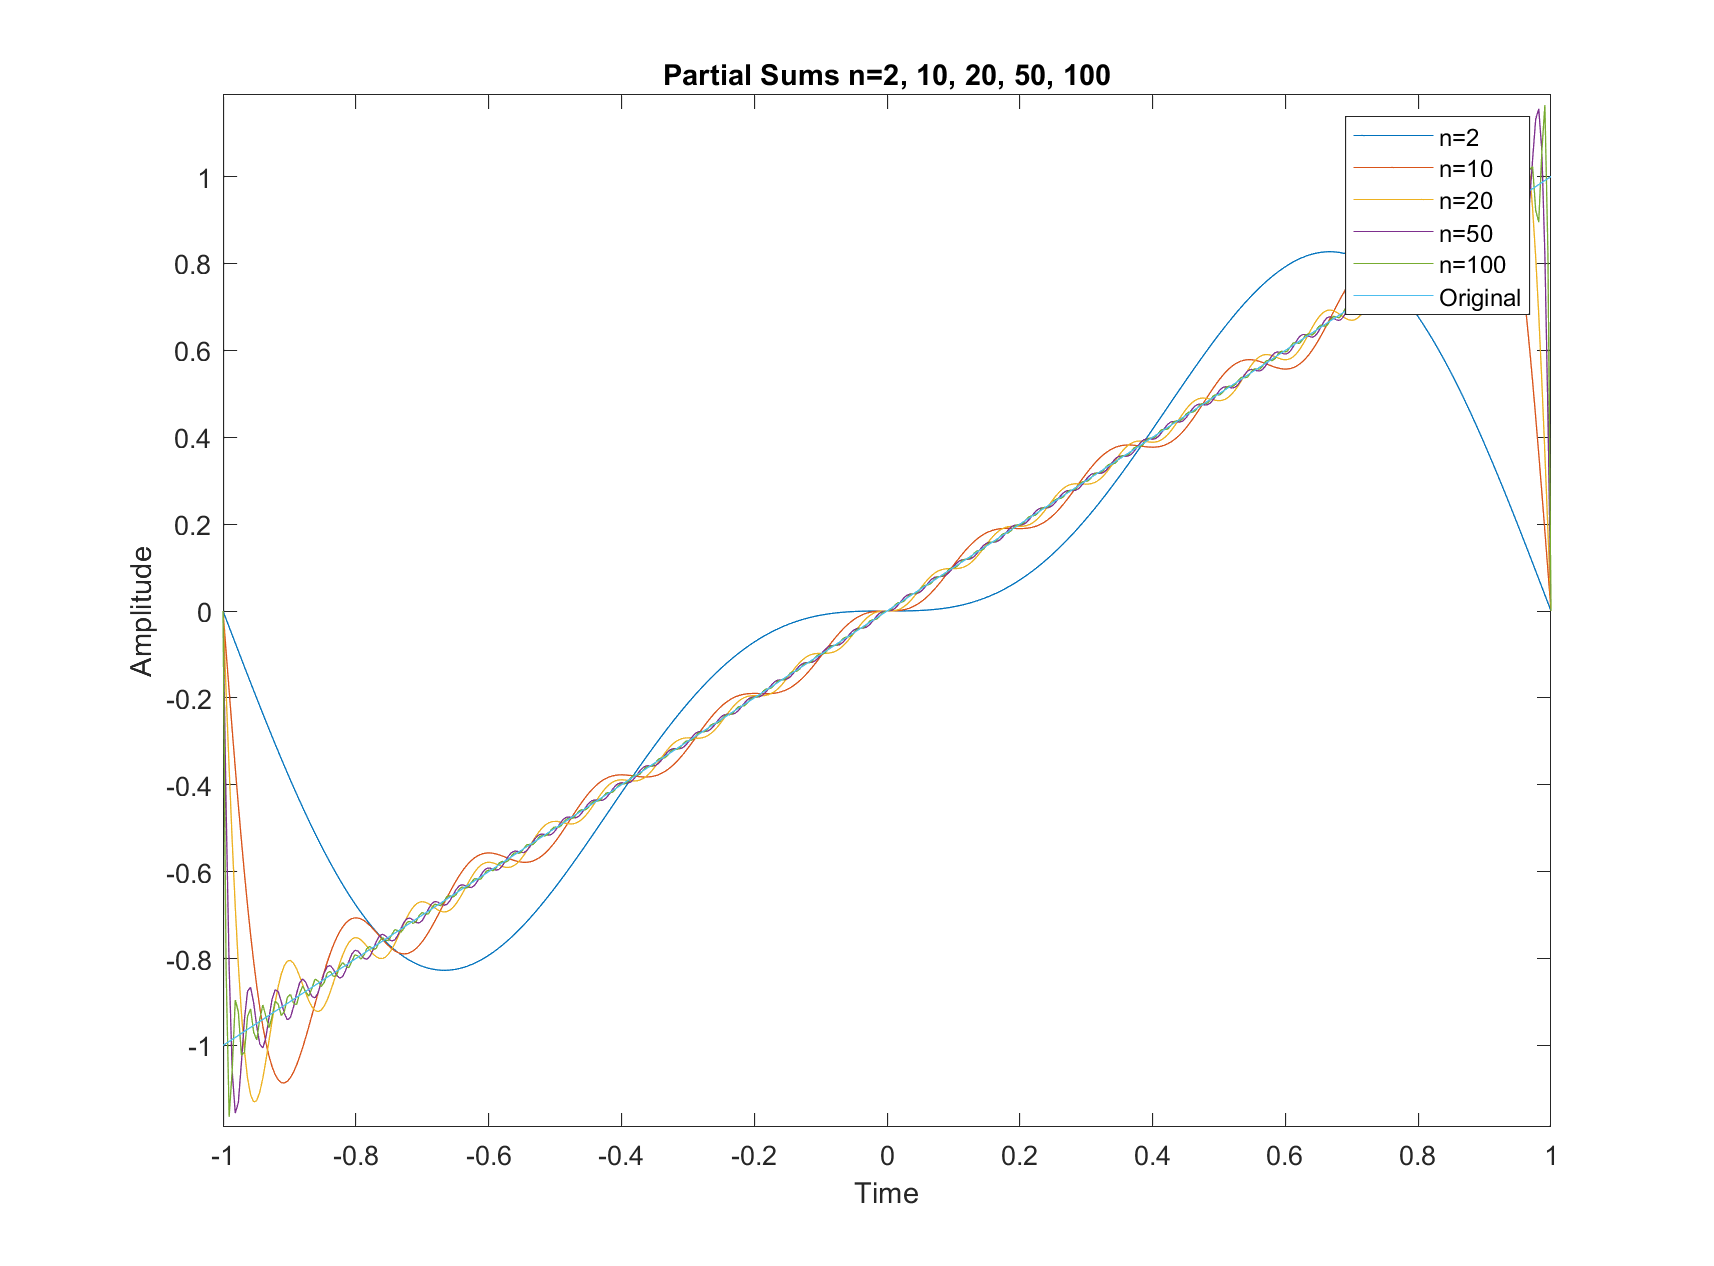
\includegraphics[width = 10cm]{linear.png}
    \caption{Trigonometric Fourier Series for \(y(t) = t\)} and \(n=10, 20, 50, 100\)
    \label{fig:linear}
\end{figure}

\section*{Exercise II}

Plot the partial sums for \(n = 10, 20, 50, 100, \text{ and } 1000\), for \(f(t) = u(t)\).

\smallskip

\textbf{Solution.}

\smallskip

\begin{lstlisting}
% Chase Lotito - ECE355L
% Exercise 2

clc
clear all
close all
syms t k L n % Initialize symbolic variables
evalin(symengine,'assume(k,Type::Integer)'); % Let matlab know that the variable k is an integer
a = @(f,t,k,L) int(f*cos(k*pi*t)/L,t,-L,L); % create kth cosine coefficient a
b = @(f,t,k,L) int(f*sin(k*pi*t)/L,t,-L,L); % create kth sine coefficient b
fs = @(f,t,n,L) a(f,t,0,L)/2 + ...
symsum(a(f,t,k,L)*cos(k*pi*t/L) + b(f,t,k,L)*sin(k*pi*t/L),k,1,n); % generate the nth partial sum
f = heaviside(t); % Original Function --> Unit Step
ezplot(fs(f,t,2,1),-1,1) % Plotting the functions and the partial sum
hold on
ezplot(fs(f,t,10,1),-1,1) % n=10
hold on
ezplot(fs(f,t,20,1),-1,1) % n=20
hold on
ezplot(fs(f,t,50,1),-1,1) % n=50
hold on
ezplot(fs(f,t,100,1),-1,1) % n=100
hold on
ezplot(fs(f,t,1000,1),-1,1) % n=1000
hold on
ezplot(f,-1,1)
hold off
title('Partial Sums n=2, 10, 20, 50, 100, 1000'),xlabel('Time'),ylabel('Amplitude')
legend('n=2', 'n=10', 'n=20', 'n=50', 'n=100', 'n=1000','Original')
\end{lstlisting}

\begin{figure}[!ht] 
    \centering
    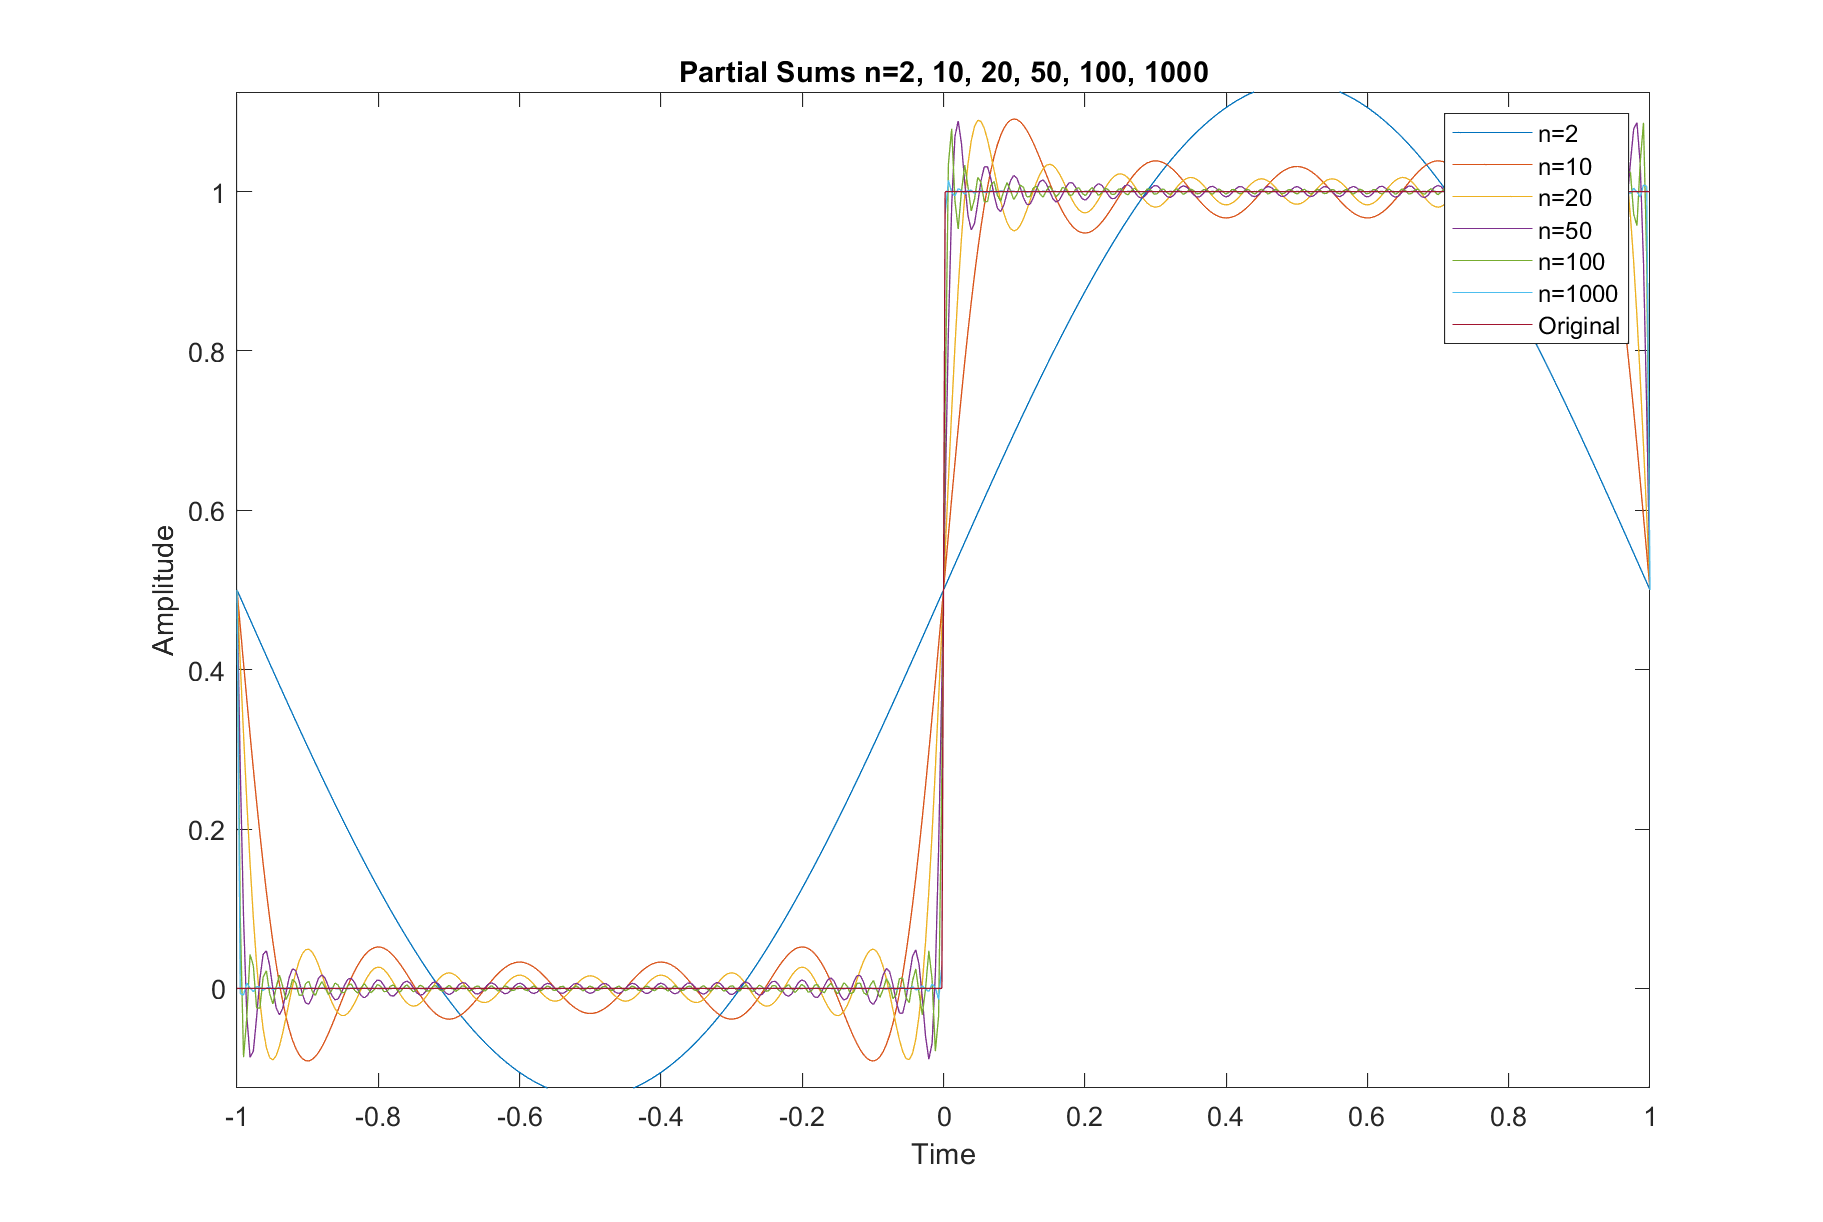
\includegraphics[width = 15cm]{unitstep.png}
    \caption{Trigonometric Fourier Series for \(y(t) = u(t)\)} and \(n=10, 20, 50, 100, 1000\)
    \label{fig:unitstep}
\end{figure}

\end{document}
